\subsection{Tính chất của đồ thị con và subdivision}

\begin{corollary}
    Đồ thị con của đồ thị phẳng là đồ thị phẳng
\end{corollary}

\begin{proof}
    Nếu $G$ là đồ thị phẳng, nghĩa là tồn tại một biểu diễn phẳng của $G$. Với mọi đồ thị con
    $H$ của $G$, ta có thể tìm đươc các đỉnh và cạnh của $H$ trong biểu diễn phẳng của $G$.
    Từ đó, ta dựng được một biểu diễn phẳng của $H$.
\end{proof}

\begin{definition}
    Subdivisions are obtained by replacing an edge with 2 edges connected by a new vertex
\end{definition}
\begin{center}
    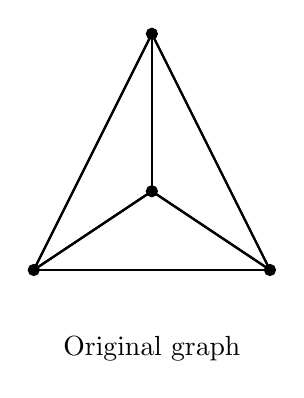
\begin{tikzpicture}
        \foreach \x/\y in {0/0, 1.5/1, 3/0, 1.5/3} {
                \filldraw[black] (\x,\y) circle (2pt);
                \foreach \z/\t in {0/0, 1.5/1, 3/0, 1.5/3} {
                        \draw[black, thick] (\x,\y) -- (\z,\t);
                    }
            }
        \node at (1.5,-1,0) {Original graph};
    \end{tikzpicture}
    \hspace{2cm}
    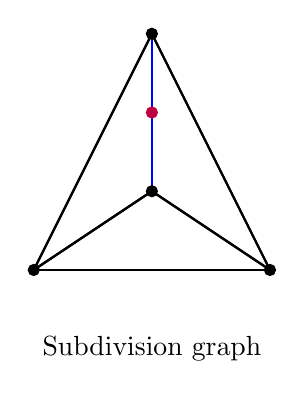
\begin{tikzpicture}
        \foreach \x/\y in {0/0, 1.5/1, 3/0, 1.5/3} {
                \foreach \z/\t in {0/0, 1.5/1, 3/0, 1.5/3} {
                        \draw[black, thick] (\x,\y) -- (\z,\t);
                    }
            }
        \node at (1.5,-1,0) {Subdivision graph};
        \draw[blue, thick] (1.5,1) -- (1.5,3);
        \filldraw[purple] (1.5,2) circle (2pt);
        \foreach \x/\y in {0/0, 1.5/1, 3/0, 1.5/3} {
                \filldraw[black] (\x,\y) circle (2pt);
            }
    \end{tikzpicture}
\end{center}

\begin{corollary}
    Subdivision của một đồ thị không phẳng là một đồ thị không phẳng.\end{corollary}
\begin{proof}
    Ai biết đâu.
\end{proof}
